\section{Case Study}\label{sec:case-study}
\frame{\tableofcontents[currentsection]}

%-------------------------------------------------
\subsection{Amusement Park}\label{subsec:amusement-park}

\begin{frame}
    \frametitle{Amusement Park}
    Amusement parks are considered to be a large business all around the world and attract people of every age and culture.

    \bigskip

   They can be considered \textit{Micro Cities} because:
    \begin{itemize}
        \item they develop in a bounded spatial area and are open daily for a given amount of hours;
        \item they offer a large set of attractions (roller-coasters, carousels, water slides, restaurants, etc.);
        \item visitors populate the park because they are interested in the attractions.
    \end{itemize}

\end{frame}
%------------------------------------------------

\subsection{Queues and Waiting Times}\label{subsec:queues-and-waiting-times}
\begin{frame}
    \frametitle{Queues and Waiting Times}
    During holidays amusement parks can get extremely busy and visitors may need to wait in long queues in order to benefit from the attractions.

    \bigskip

    \begin{center}
        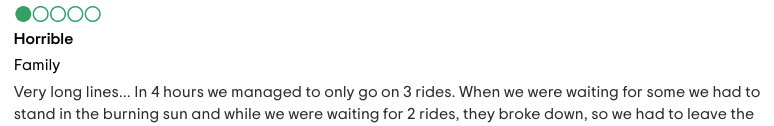
\includegraphics[width=0.7\textwidth]{../img/review1}
        \label{fig:review1}
    \end{center}

    \smallskip

    \begin{center}
        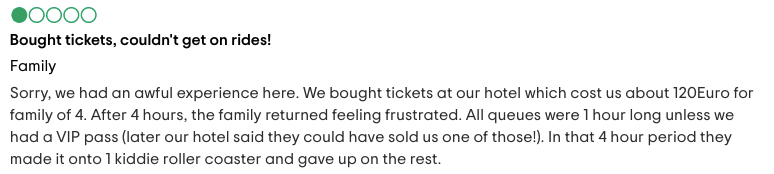
\includegraphics[width=0.7\textwidth]{../img/review2}
        \label{fig:review2}
    \end{center}

    \bigskip

    This can have a very bad impact on visitors' experience\ldots

\end{frame}
%------------------------------------------------

\subsection{Recommendation and Rewards}\label{subsec:recommendation-and-rewards2}
\begin{frame}
    \frametitle{Recommendation and Rewards}
    In this scenario the \textit{situated recommendation system} could suggest the most suitable attraction for the visitors, taking into account information such as how busy the attractions are and which attractions the single visitor is interested in.
\end{frame}

\subsection{Requirements}\label{subsec:requirements}
\begin{frame}
    \frametitle{Requirements}
    In order to be appealing to amusement parks, the \textit{situated recommendation system should}:
    \begin{itemize}
        \item \textbf{make recommendations} based on certain criteria.
        It should abstract from the particular strategy used to calculate the recommendations;
        \item \textbf{track the state of every attraction} inside the park in order to provide dynamic and \textit{context-aware} recommendations;
        \item \textbf{track the state of every visitor} (or group of visitors) in order to provide them with \textit{situated} and personalized recommendation;
        \item memorize the information collected during the park's lifetime in order to develop more and more effective recommendation strategies.
    \end{itemize}
\end{frame}
